\documentclass[12pt,a4paper]{report}
\usepackage[english,brazilian]{babel}
\usepackage[utf8]{inputenc}
\usepackage[T1]{fontenc}
\usepackage{amsmath,amsthm,amsfonts,amssymb,textcomp}
%\usepackage{latexsym}
\usepackage{graphicx}
\graphicspath{{figuras}}
\usepackage{subfigure}
\usepackage{float}
\usepackage{longtable}
\usepackage{color}
\usepackage{epstopdf}
\usepackage{pdflscape}
\usepackage[breaklinks=true]{hyperref}
\usepackage[comma,authoryear]{natbib}
\usepackage[nonumberlist]{glossaries}
\usepackage{arydshln}
%\usepackage{floatrow}
\usepackage{footnote}
\usepackage[left=3cm,right=2cm,top=3cm,bottom=2cm]{geometry}
%\usepackage{blindtext}

%\usepackage[alf]{abntcite}

%%% newcommand %%%%%%%%%%%%%%%%%
\newcommand{\PE}{Perkin-Elmer}
\newcommand{\BC}{Boller \& Chivens}

\newcommand{\degr}{\ensuremath{^{\circ}}}%                    % degree symbol:  °
\newcommand{\arcmin}{\ensuremath{^{\prime}}}%                    % degree symbol:  °
\newcommand{\arcsec}{\ensuremath{^{\prime\prime}}}%                    % degree symbol:  °
\newcommand{\fs}{\mbox{\ensuremath{.\!\!^s}}}
\newcommand{\farcm}{\mbox{\ensuremath{.\mkern-4mu^\prime}}}%    % fractional arcminute symbol: 0.'0
\newcommand{\farcs}{\mbox{\ensuremath{.\!\!^{\prime\prime}}}}%  % fractional arcsecond symbol: 0.''0
\newcommand{\fdg}{\mbox{\ensuremath{.\!\!^\circ}}}%             % fractional degree symbol:     0.°0
%\newfloatcommand{capbtabbox}{table}[][\FBwidth]




%\makeglossaries

\makeatletter
\renewcommand\chapter{\thispagestyle{plain}
                \global\@topnum\z@
                \@afterindentfalse
                \secdef\@chapter\@schapter}
\makeatother


\makeatletter
\renewcommand{\@makechapterhead}[1]{%
\vspace*{20 pt}%
{\setlength{\parindent}{0pt} \raggedright \normalfont
\bfseries\Large\thechapter.\ #1
\par\nobreak\vspace{8 pt}}}
\makeatother

%\newglossaryentry{Offset}{name={Offset}, description={Diferença entre a posição obtida pela redução da observação e a posição dada pela efeméride}}
\newglossaryentry{OPD}{name={OPD}, description={Observatório do Pico dos Dias - Brasópolis, MG}}
\newglossaryentry{LNA}{name={LNA}, description={Laboratório Nacional de Astrofísica - Itajubá, MG}}
\newglossaryentry{OHP}{name={OHP}, description={Observatoire Haute Provence - Saint-Michel-l'Observatoire, França}}
\newglossaryentry{RA}{name={RA}, description={Sigla para Ascensão Reta ($ \alpha $)}}
\newglossaryentry{DEC}{name={DEC}, description={Sigla para Declinação ($ \delta $)}}
\newglossaryentry{Anomalia Verdadeira}{name={Anomalia Verdadeira}, description={Ângulo formado entre o Periastro e a posição instantânea do objeto na órbita centrado no planeta e contada na direção do movimento orbital}}
\date{}
\author{Altair Ramos Gomes Júnior}
\title{Relatório das Atividades de PG 2015-2016}
\begin{document}

\maketitle

%\pagestyle{headings}

\chapter{Introdução}
\label{Cap: intro}

\indent \indent O Sistema Solar, apesar de próximo, em um âmbito astronômico, ainda não é completamente conhecido. Uma de suas surpresas mais recentes, por exemplo, foi a descoberta de um sistema de anéis ao redor do Centauro Chariklo \citep{BragaRibas2014}, característica nunca antes observada em um objeto que não fosse um planeta gigante.

Objetos como Centauros, Objetos Trans-Netunianos (TNOs) e satélites irregulares estão localizados a grandes distâncias do Sol, em regiões de baixa temperatura. Portanto, comparados a objetos formados mais próximos do Sol, eles provavelmente sofreram pouca diferenciação, seja por mecanismos internos ou por colisões frequentes (choques reais ou passagens gravitacionalmente próximas) com outros objetos.

Acredita-se, por isso, que os TNOs guardam estruturas e composições relativamente inalteradas de sua época de formação. Portanto eles são muito importantes para estudar a formação do Sistema Solar. Tirando Plutão, o primeiro TNO foi descoberto há pouco mais de 20 anos \citep{Jewitt1993}. Por isso, as propriedades básicas desta população ainda não estão inteiramente estabelecidas, como a distribuição de tamanhos, composição, estruturas internas.

Centauros são uma população transiente entre TNOs e cometas da família de Júpiter, orbitando em uma região entre Júpiter e Netuno. Uma vez que Centauros são tipicamente mais brilhantes que TNOs por estarem mais próximos, eles servem como representantes a partir dos quais é possível inferir propriedades mais gerais sobre os objetos mais distantes \citep{Fernandez2002}.

Segundo o modelo de Nice \citep{Morbidelli2005,Gomes2005,Tsiganis2005}, muitos dos objetos que pertenciam ao cinturão de Kuiper primordial acabaram sendo enviados pela interação com os planetas gigantes para as partes mais internas do Sistema Solar. Alguns podem ter sido capturados pelos planetas criando a população de satélites irregulares ou satélites externos \citep{Nesvorny2007}, troianos \citep{Morbidelli2005} ou até mesmo para o cinturão principal de asteroides como proposto para Ceres por \cite{McKinnon2012}, hipótese reforçada por resultados recentes \citep{DeSanctis2015} a partir de observações da sonda \textit{Dawn}. Estudar esses objetos é de grande importância para entender a evolução do Sistema Solar.

Desses objetos, Tritão possui um interesse particular. Ele foi capturado por Netuno \citep{McKinnon2007} em uma órbita retrógrada e próxima ao planeta. Sua superfície é deformada com características tectônicas e possivelmente criovulcânicas \citep{Nimmo2015} e as propriedades físicas já conhecidas de Tritão mostram uma similaridade com as de Plutão. Além do mais, é um dos poucos objetos do Sistema Solar que se sabe possuir atmosfera.

Com exceção dos planetas gigantes e seus satélites internos, apenas Plutão e Phoebe, satélite irregular de Saturno, foram observados, com grande qualidade de dados, por sondas espaciais além da órbita de Júpiter. Por isso, ainda hoje, as observações de solo tem se mostrado de grande importância.

Um método que tem se mostrado eficiente para a obtenção desses parâmetros é o método de ocultações estelares, que proporciona medidas tão precisas que são apenas superadas por medidas oriundas de sondas. De fato, a sonda \textit{Dawn} já está orbitando Ceres e a sonda \textit{New Horizons} visitou Plutão \citep{Stern2015}. As observações feitas por essas sondas trazem a oportunidade perfeita para comparar os resultados com os obtidos pelas nossas ocultações e calibrar a técnica, de forma que ocultações feitas para outros objetos possam ser ainda mais precisas.

O objetivo desse Doutorado é observar objetos do Sistema Solar exterior, fazer astrometria para melhorar suas efemérides de forma que ocultações estelares por esses objetos possam ser preditas com precisão, observar as ocultações e obter os parâmetros físicos.

Assim, além do trabalho rotineiro de estudo de TNOs e Centauros feito pelo grupo, do qual eu participo ativamente, nos propomos a estudar aqui, no contexto observacional acima, alguns objetos que, por hipótese, também podem ser representativos da população original de TNOs, isto é, podem ter uma origem comum aos TNOs. São eles alguns dos satélites irregulares de planetas gigantes, Ceres e Tritão.


%\chapter{Centauros e TNOs}
%\label{Cap: TNOs}

%\section{Introdução}
%\label{Sec: TNOs-intro}

%\indent \indent Dentro do contexto explicitado no capítulo \ref{Cap: intro}, os TNOs são uns dos objetos mais significantes por possivelmente serem a fonte de outras populações do Sistema Solar, como por exemplo Centauros \citep{Fernandez2002}, Satélites Irregulares \citep{Nesvorny2007} e Troianos \citep{Morbidelli2005}. Também existe a possibilidade de que Ceres tenha uma origem como TNO \citep{McKinnon2012}, assim como Tritão \citep{Agnor2006}.

%Pouco se conhece sobre Centauros e TNOs, pois nunca foram visitados por sondas, com a exceção de Plutão, e a grande maioria das observações são de origem fotométrica usual (magnitudes, cores) ou, em menor parte, espectroscópica, ou em menor número ainda por telescópios espaciais.

%Estimar parâmetros físicos como tamanho, albedo, densidade, etc para esses objetos é um desafio, porém essencial para acessar a massa atual e composição (material) da população e recuperar sua história evolutiva. %É possível obter seus tamanhos através de modelos, por exemplo combinando o brilho no visível e emissão térmica obtida em infra-vermelho. Todavia os erros obtidos são piores que 10 \% \citep{Camargo2013}.
%Para se obter esses parâmetros, de forma muito precisa e acurada, sem a necessidade de se adotar modelos, utilizamos a técnica de ocultações estelares. Até 2009, quando foi observada uma ocultação de 2002TX300 \citep{Elliot2010}, Plutão e Caronte eram os únicos TNOs com ocultações observadas. Até hoje, cerca de uma dezena de TNOs e Centauros tiveram ocultações observadas.%, alguns com apenas uma corda, como Varuna, o que permite apenas determinar um tamanho mínimo para o objeto.

%Com o objetivo de prever e observar ocultações estelares por TNOs, o nosso grupo conta com colaboração de pesquisadores nacionais e internacionais, profissionais e amadores. Utilizamos telescópios de pequeno e grande porte e câmera rápida para observar eventos que proporcionaram grandes descobertas, como por exemplo a descoberta do sistema de anéis ao redor do Centauro Chariklo \citep{BragaRibas2014}.



\chapter{Ocultações Estelares}
\label{Cap: Occ}

\indent \indent Uma ocultação estelar ocorre quando um objeto do Sistema Solar passa em frente a uma estrela. A sombra causada por esse fenômeno passaria sobre a Terra e um observador que estivesse sob essa sombra veria uma variação no brilho do par objeto-estrela ao longo do tempo. A curva de luz oriunda da ocultação pode ser usada para inferir parâmetros físicos como tamanho, albedo, densidade, etc, para o objeto ocultante.

Com várias curvas de luz observadas no mesmo evento e obtidas em diferentes regiões da sombra se pode obter a forma e tamanho do objeto. Conhecendo-se a magnitude absoluta, calcula-se o albedo. Se a massa é conhecida, calcula-se sua densidade. Atmosferas e anéis também podem ser descobertos por esse método.

\section{TNOs}
\label{Sec: TNO-occ}

Até 2009, quando foi observada uma ocultação de 2002TX300 \citep{Elliot2010}, Plutão e Caronte eram os únicos TNOs com ocultações observadas. Até hoje, cerca de uma dezena de TNOs e Centauros tiveram ocultações observadas.

Observar uma ocultação estelar exige um grande trabalho de predição e de sua melhoria. Os TNOs estão muito distantes significando que mesmo sem grandes erros nas suas efemérides ou na posição da estrela o erro do local por onde a sombra irá passar pode ser de milhares de quilômetros. Preferencialmente, esse erro tem que ser menor que o tamanho angular do objeto no plano do céu. Por exemplo, Plutão tem um raio de $1190 \pm 5$ km \cite{DiasOliveira2015} que a uma distância de aproximadamente 32 UA representa um diâmetro angular de 102 mas. Para a maioria dos objetos selecionados, menores que Plutão e/ou mais distantes, seus tamanhos angulares são menores que 50 mas.

Devido ao grande esforço necessário para se prever e observar ocultações estelares (a sombra do objeto pode passar em qualquer lugar na Terra) e o interesse científico que o método proporciona, o nosso grupo conta com colaboração de pesquisadores nacionais e internacionais, profissionais e amadores. Utilizamos telescópios de pequeno e grande porte e câmera rápida para observar eventos que proporcionaram grandes descobertas, como por exemplo a descoberta do sistema de anéis ao redor do Centauro Chariklo \citep{BragaRibas2014}, do qual colaborei.

Dentro do meu programa de doutorado, participei e participo ativamente na observação e redução astrométrica de TNOs e estrelas a serem ocultadas. Essas observações são utilizadas na melhoria das predições dos eventos diminuindo erros na localização na Terra onde a sombra passaria.

Até há pouco tempo um grande esforço era feito para melhorar as posições das estrelas uma vez que o melhor catálogo de estrelas de referência disponível, o UCAC4 \citep{Zacharias2013}, tinha erros maiores do que o necessário para uma boa predição. Porém, recentemente tivemos o primeiro release do catálogo GAIA \citep{Brown2016}, que proporcionará melhores posições para as estrelas, na casa dos micro-segundos de arco.

Não somente as posições das estrelas precisam ser atualizadas, mas também as posições dos TNOs. Portanto os TNOs também foram observados tanto no ESO quanto no Observatório do Pico dos Dias. %(OPD, LNA/MCTI, Itajuba, MG., código IAU 874, $45^{\circ} ~34\arcmin ~57\arcsec$ W, $22^{\circ} ~32\arcmin ~04\arcsec$ S, 1864 m).
A princípio as predições das ocultações eram atualizadas utilizando o método de offsets, porém, em colaboração com o Dr. Josselin Desmars, integrações numéricas das órbitas dos TNOs foram realizadas desenvolvendo-se uma ferramenta denominada NIMA\footnote{Numerical Integration of the Motion of an Asteroid}, cuja publicação \citep{Desmars2015} sou co-autor.


Uma grande campanha observacional é realizada para se observar ocultações estelares por TNOs e Centauros. Essa campanha é liderada por pesquisadores brasileiros, franceses e espanhóis e tem colaboração com observadores espalhados por todo o mundo resultando em vários objetos já observados. As observações bem sucedidas de ocultações estelares resultantes desse trabalho de predição já geraram diversas publicações, inclusive na revista Nature, por exemplo \cite{Sicardy2011} e \cite{BragaRibas2014} nas quais contribuí em caráter observacional. A ocultação de Plutão de 04 de Maio de 2013, a qual observei, gerou duas publicações \citep{Olkin2015, DiasOliveira2015}.

\cite{Sicardy2011} identificaram, a partir de uma ocultação de 06 de Novembro de 2010, que Eris é um planeta anão menor do que se esperava. Devido a seu brilho e distância acreditava-se que ele fosse muito maior, mas na verdade ele tem um albedo geométrico no visível de $p_v=0.96^{+0.09}_{-0.04}$ e seu tamanho é de $1163 \pm 6$ km, muito próximo ao tamanho de Plutão. O alto albedo de Eris pode ser relacionado à presença de uma atmosfera colapsada devido ao fato dele estar se aproximando de seu afélio.

\cite{BragaRibas2014} observaram uma ocultação do Centauro Chariklo que ocorreu dia 03 de Junho de 2013. O ocultação revelou que o objeto possui um sistema de anéis nunca visto antes em um objeto tão pequeno. Até o momento, conhecia-se apenas anéis em torno dos planetas gigantes. Essa descoberta levanta muitas questões sobre formação dos anéis, estabilidade e tempo de vida e nos leva a crer que pode haver mais objetos com anéis no Sistema Solar, ao menos nessa região.

\cite{Olkin2015} determinaram a partir de observações de ocultações por Plutão que a atmosfera do objeto não colapsa durante os 248 anos de sua órbita, como acontece com Eris. Modelos anteriores previam um colapso de sua atmosfera devido a Plutão receber três vezes menos luz do Sol em afélio que em seu periélio.

\cite{DiasOliveira2015}, também a partir de ocultações de Plutão, utilizaram modelos para obter os perfis de temperatura, pressão e densidade da atmosfera do objeto. Os modelos ajustam perfeitamente os perfis de temperatura para as duas ocultações utilizadas assumindo uma atmosfera esfericamente simétrica. Por fim, foi obtido que a pressão da atmosfera aumentou cerca de 6\% entre 2012 e 2013 significando que a atmosfera de Plutão ainda está se expandindo e confirmando o trabalho de \cite{Olkin2015}.

Além desses contribuí com outras ocultações como a de Plutão observada na Austrália e Nova Zelândia em 29 de Junho de 2015 e a de Chariklo em 29 de Abril de 2014 reduzindo curvas de luz, observei uma ocultação do TNO 2003VS2 dia 07 de Novembro de 2014 no OPD e trabalhei na predição de eventos como os dos TNOs 2003AZ84 e 2006UK126. Alguns desses trabalhos ainda não foram publicados.

\cite{Sicardy2016} obteve os perfis de atmosfera para Plutão a partir do evento do dia 29 de Junho de 2015 Esse evento foi de máxima importância devido a esta ser a última antes da chegada da sonda \textit{New Horizons} no sistema e foi observada na Austrália e Nova Zelândia. Os modelos de perfil de atmosfera para Plutão poderão ser calibrados com os dados da \textit{New Horizons} para serem utilizados em futuras ocultações e estudar a evolução da atmosfera do planeta anão.

\cite{Alex2016}, submetido, identificou no TNO 2003AZ84 uma possível fenda através de uma ocultação que ocorreu em 3 de Fevereiro de 2014. Ocasionalmente, uma das cordas do evento foi observada na borda da sombra. Esse não é o primeiro objeto com fenda a ser descoberto nessa região. Na verdade, a sonda \textit{New Horizons} observou uma fenda de grandes proporções no maior satélite de Plutão, Caronte \citep{Stern2015}.

\cite{Rossi2016}, aceito, publicou resultados da ocultação do TNO 2007UK126. Essa foi a primeira ocultação observada pelo projeto RECON. Esse projeto possui diversos telescópios que foram espalhados pela costa oeste dos Estados Unidos. A importância desse grupo se deve à grande área que ele cobre. Isso possibilitará que diversos outros eventos possam ser observados com grande qualidade espacial.


\section{Ceres}
\label{Sub: Ceres}

\indent \indent Apesar de Ceres não ser um objeto do Sistema Solar exterior, ele é o único planeta-anão no Sistema Solar interno e, por isso, é um objeto de grande importância e seu estudo pode ter grande impacto na formação e evolução do Sistema Solar. Na verdade, foi proposto que a origem de Ceres pode ser comum aos objetos trans-Netunianos \citep{McKinnon2012}, espalhado posteriormente para o cinturão principal de asteroides devido à migração dos planetas gigantes predito pelo Modelo de Nice \citep{Gomes2005}.

\cite{DeSanctis2015} reforça essa teoria. A partir do observações do espectrômetro VIMS da sonda \textit{Dawn} ele identificou filossilicatos amoniados presentes na superfície de Ceres. Como amônia é mais abundante no Sistema Solar Exterior, o trabalho sugere que Ceres ou tem uma origem nessa região ou ele acretou muito material que foi transportado para o Cinturão Principal de Asteroides.

Contendo aproximadamente um quinto de toda a massa do cinturão de asteroides, espera-se que Ceres esteja em equilíbrio gravitacional e seja, portanto, um elipsoide Maclaurin ou Jacobi. De fato, observações diretas de Ceres com a utilização de ótica adaptativa indica que ele é um esferoide achatado nos polos \citep{Drummond2014}. O conhecimento preciso de seu tamanho e forma é de extrema importância para modelos de densidade, estrutura interna e diferenciação.

Com este fim, foram preditos dois eventos por Steve Preston\footnote{Predições publicadas em \url{http://asteroidoccultation.com}.} para a IOTA (International Occultation Timing Association), durante predições de rotina de ocultações de estrelas brilhantes por asteroides. As ocultações desse objeto me renderam uma publicação como primeiro autor, \citep{GomesJunior2015-Ceres}.

%Foram preditos dois eventos por Steve Preston\footnote{Predições publicadas em \url{http://asteroidoccultation.com}.} para a IOTA (International Occultation Timing Association), durante predições de rotina de ocultações de estrelas brilhantes por asteroides.

O primeiro evento foi observado no Brasil em 17 de Agosto de 2010 em cinco diferentes sítios. Destes, 4 obtiveram cordas positivas enquanto UFSC teve corda negativa. Das positivas, a observação proveniente do INPE iniciou-se após o início do evento devido a dificuldades técnicas e, portanto, apenas a emersão da curva de luz foi detectada. O segundo foi observado no do dia 25 de Outubro de 2013 na costa Leste dos Estados Unidos.

As curvas de luz de cada observação foram obtidas das imagens FITS com a utilização do pacote PRAIA \citep[Plataforma de Redução Astrométrica de Imagens Astronômicas,][]{Assafin2011}. O evento de 2010 foi reduzido pelo Felipe Braga Ribas enquanto eu reduzi o evento de 2013. Os instantes de ingresso e egresso foram obtidas de cada curva de luz ajustando-se um modelo de poço quadrado levando em consideração a difração de Fresnel, a banda do CCD, o diâmetro aparente da estrela e o tempo de exposição utilizado \citep[ver][]{Widemann2009, Braga-Ribas2013}. Algumas cordas do evento de 2013 não foram utilizadas por haver erros nos tempos fornecidos identificados durante o tratamento das imagens.

Duas possíveis soluções foram consideradas para o ajuste do limbo. A primeira, que chamamos de solução nominal, consiste em determinar os cinco parâmetros que caracterizam uma elipse a partir dos contatos observados. A segunda consiste em calcular o ângulo de posição $P$ a partir das coordenadas do polo de Ceres obtidas por \cite{Drummond2014} ($\alpha_{p} = (287 \pm 3) \degr$, $\delta_{p} = (+64 \pm 3) \degr$ no ICRS) e da efeméride de Ceres no instante da ocultação. Chamamos de solução de polo fixo.

O evento de 2010, por exemplo, teve somente sete contatos, porém bem distribuídos sobre o disco de Ceres. Por outro lado, o evento de 2013 teve cinco contatos a mais, todavia concentrados em certas regiões do corpo. Em particular, a ausência de cordas próximas ao polo sul fez seu achatamento ser pior determinado para o evento de 2013 que para o evento de 2010. Mesmo nossa melhor medida de achatamento, $\epsilon=0.08 \pm 0.03$, tem alta incerteza se comparado com outros valores publicados na literatura.

Usar as coordenadas do polo de Ceres determinadas por \cite{Drummond2014} para limitar o ângulo de posição não foi um procedimento eficiente para o evento de 2013. Por outro lado, reduziu as barras de erro dos outros parâmetros (com exceção do achatamento) para a ocultação de 2010. Por fim, esse procedimento resultou em um excelente acordo entre os raios equatoriais obtidos para ambos os eventos.

Uma comparação do diâmetro equatorial de Ceres medido por diferentes técnicas mostra um acordo entre os nossos resultados e aqueles obtidos por imageamente direto do Hubble Space Telescope (HST) \citep{Thomas2005}, do Keck Observatory e do ESO VLT \citep{Drummond2014}.

A sonda da NASA \textit{Dawn} chegou e está obtendo dados de Ceres desde o começo de 2015 \citep{Russell2016}. Seus resultados poderão elucidar muitas perguntas sobre Ceres e serão utilizados para calibrar todas as técnicas usadas até agora para o estudo das propriedades físicas dos pequenos objetos do Sistema Solar, como as ocultações estelares.

O resultado deste trabalho foi publicado em \cite{GomesJunior2015-Ceres}.

%\newpage
\chapter{Satélites Irregulares dos planetas gigantes}
\label{Cap: Irregulares}

\section{Introdução}
\label{Sec: Irr-intro}

\indent \indent Os satélites irregulares, também denominados satélites externos, dos planetas gigantes são menores que os regulares, possuindo órbitas mais excêntricas, inclinadas e distantes. Na maioria dos casos, essas órbitas são retrógradas. Devido a suas configurações orbitais, é amplamente aceito que estes objetos foram capturados nos estágios iniciais da formação do Sistema Solar \citep{Sheppard2003}.

Por serem relativamente pequenos, eles são pouco brilhantes e só foram descobertos no último século. Dentre os satélite irregulares dos planetas gigantes, poucos são aqueles que possuem medidas de seus parâmetros físicos. Apenas Himalia, Phoebe e Nereida foram observados por sondas, apesar de não serem medidas ideais, já que foram alvos de oportunidade. Destes apenas Phoebe teve seu tamanho estimado a partir de imagens de alta resolução da Cassini com um erro médio de 0.7 km.

Se esses objetos foram capturados, permanece a pergunta de onde eles vieram. Estudos como os de \citealp{Grav2003, Clark2005} e \citealp{Grav2007} mostraram através de suas cores e inclinações espectrais que esses satélites contêm uma fração mais ou menos igual de objetos semelhantes a asteroides tipo C, P e D ou a Centauros e TNOs. Esses trabalhos sugerem origens diferentes para os satélites irregulares.

Nesse contexto, durante o Mestrado, foi realizado junto ao grupo um trabalho astrométrico para a melhoria das efemérides dos satélites irregulares de Júpiter e Saturno. Em colaboração com o Dr. Jean-Eudes Arlot do IMCCE, reduzi um banco de dados observado no Observatoire Haute-Provence (OHP) entre 1998 e 2008, contendo mais de 28 mil posições para 10 satélites. Reduzi também um banco de dados com mais de 100 mil imagens obtidas no Observatório do Pico dos Dias (OPD) entre 1992 e 2014. Já no Doutorado, neste mesmo âmbito, reduzi 810 observações feitas no European Southern Observatory (ESO) em 24 noites utilizando o detector mosaico CCD Wide Field Imager (WFI).

Um total de 6523 posições de 18 satélites foram identificadas. Esse trabalho está publicado \citep{GomesJunior2015-Irregular} e o catálogo com as posições está disponível no CDS. Um dos principais resultados obtidos foi a grande quantidade de posições identificadas para os satélites irregulares em comparação com a quantidade utilizada nas integrações numéricas atuais publicadas por \cite{Jacobson2012}. Dessa forma, é de se esperar que nossas posições contribuam significativamente para a melhoria da órbita desses objetos.

Observando os offsets das posições com respeito às efemérides ao longo do tempo e anomalia verdadeira foram identificados erros sistemáticos nas efemérides. O erro mais evidente é na declinação do satélite Carme o qual foi associado a um erro em sua inclinação orbital. Esse padrão em declinação também foi identificado para outros satélites como Pasiphae e Ananke. Para alguns satélites a cobertura orbital não foi suficiente para indicar claramente a presença de erros sistemáticos em elementos orbitais específicos. Os gráficos para todos os satélites estão disponíveis em \cite{GomesJunior2015-Irregular}.


\section{Predição das ocultações}
\label{Sec: Irr-predic}

\indent \indent Com o objetivo de obter parâmetros físicos para os satélites irregulares com maior precisão foram feitas predições de ocultações estelares para os 8 maiores satélites de Júpiter (Himalia, Elara, Pasiphae, Sinope, Lysithea, Carme, Ananke e Leda) e o satélite Phoebe de Saturno. Esses objetos são pequenos, se comparados aos TNOs estudados na seção \ref{Sec: TNO-occ}, sendo que o menor dos satélites da amostra, Leda, possui um diâmetro estimado de 20 km.

As predições foram feitas utilizando as posições de estrelas dadas no catálogo UCAC4. Para as posições dos satélites de Júpiter foi feita uma nova integração numérica utilizando as posições publicadas em \cite{GomesJunior2015-Irregular}. Essa integração foi realizada pela pós-doc do grupo no ON Laurène Beauvalet. Outras posições publicadas na literatura não foram utilizadas. Isso se deve por não estarmos interessados em efemérides a longo prazo uma vez que só faremos predições até o fim de 2020. Além disso, a confiança que temos nos nossos dados é muito maior, e analisar as posições de outros observadores exigiria muito tempo e esforço fora do escopo do trabalho.

Para Phoebe atualizamos as efemérides publicadas por \cite{Desmars2013} adicionando as posições de \cite{GomesJunior2015-Irregular}, \cite{Peng2015}, MPC e Flagstaff. Um total de 5886 posições foram utilizadas. Isso representou um acréscimo de cerca de 75\% em comparação à \cite{Desmars2013}, a maioria com observações recentes, o que é requerido ao nosso propósito.

Aproximadamente 5442 eventos foram obtidos entre 01 de Janeiro de 2016 e 31 de Dezembro de 2020 para os 9 objetos. A maioria será descartada por passar em regiões de oceano ou onde não há observadores disponíveis. Estima-se que restem ao final cerca de 10\% desse número.

A razão desse grande número de eventos se deve ao fato que Júpiter, em seu caminho aparente no céu, irá passar pelo plano da galáxia em 2019-2020 e Saturno em 2018. Devido à grande densidade de estrelas nessa região, o número de eventos por ano é cerca de 15 vezes maior do que quando fora dessa região. Por exemplo Carme, com 20 ocultações previstas em 2016, ocultará 369 estrelas em 2019.

Como esses objetos são muito pequenos, em sua maioria as ocultações durarão poucos segundos, portanto apenas eventos com estrelas brilhantes serão selecionados e se houver câmeras de integração rápida disponíveis. Por outro lado, os satélites de Júpiter estão muito mais perto que os TNOs e como o erro astrométrico é uma medida angular, consequentemente, o erro da sombra da ocultação projetada na Terra será muito menor que para TNOs. Assim, as latitudes a serem cobertas para que uma ocultação por satélite irregular de Júpiter seja detectada corresponde a poucas centenas de quilômetros. Destes, cerca de 10\% dos eventos envolvem estrelas mais brilhantes de magnitude R=14 e 25\% mais brilhantes que R=15. Isso facilitará a observação por observadores amadores.

Até o momento, dois testes de ocultações foram feitos, um de Himalia que ocorreu dia 03 de Março de 2015 e o segundo de Elara que ocorreu dia 30 de Março de 2015. Foram comparadas predições oriundas da nossa integração numérica, das efemérides do JPL, e de offsets de observações tomadas próximas à data do evento.

Para o evento de Himalia identificamos uma boa concordância entre as predições. De fato, a maior diferença entre as sombras calculadas é de $25 s$ e $130 km$ na direção perpendicular às sombras. Para o evento de Elara as observações tomadas no Zeiss prejudicaram a qualidade das posições uma vez que Elara é um objeto pouco brilhante. Ainda assim, as diferenças entre os mapas obtidos foram relativamente pequenas. A maior diferença entre elas é de $48 s$ e $302 km$.

Uma ocultação de Himalia, maior satélite irregular de Júpiter, estava prevista para 23 de Outubro de 2015 quando a sombra passaria no Brasil. As condições não eram muito propícias. A estrela possuía magnitude R=15.5, os objetos estavam baixo no céu, cerca de 30 graus de altura, e próximo ao amanhecer.

De toda forma, organizei junto com o Dr. Felipe Braga Ribas, do Instituto Tecnológico Federal do Paraná, uma campanha para a observação do evento. Reunimos observadores em Guaratinguetá-SP, São Paulo-SP, Valinhos-SP, Vitória-ES, Brasília-DF, Curitiba-PR, Ponta-Grossa-PR, Oliveira-MG e no Observatório do Pico dos Dias. No fim das contas, todos os observadores não puderam observar o evento devido ao mau tempo.

Também foram feitas predições para Sycorax, satélite irregular de Urano, e Nereida, satélite irregular de Netuno. Porém, dentro do intervalo de 5 anos pesquisado, apenas 2 eventos por satélite foram identificados. Isso se deve ao fato de Urano e Netuno estarem passando por uma região pouco densa de estrelas no céu. Como esses eventos apresentavam más condições de observação, estrela fraca, sombra passando pelo oceano, etc., eles não foram incluídos no trabalho.

A próxima etapa é atualizar as predições feitas com o UCAC4 utilizando as posições GAIA, cujo primeiro release se deu em setembro de 2016 \citep{Brown2016}. A falta de movimentos próprios no release I não afetará as predições uma vez que estas tem datas próximas à data de observação do GAIA (época média do catálogo).

O trabalho de predições usando o catálogo UCAC4, junto com tabelas de informações sobre os eventos, foi publicado por \cite{GomesJunior2016}. Essas predições também são disponibilizadas na rede \textit{OccultWatcher}\footnote{http://www.occultwatcher.net/} onde podem ser visualizadas por observadores, em sua maioria amadores, em todo o mundo.


\chapter{Netuno e Tritão}
\label{Cap: Netuno-Tritao}

%\section{Introdução}
%\label{Sec: Netuno-intro}

\indent \indent Tritão é um satélite de Netuno que, diferentemente dos satélites regulares dos outros planetas, possui uma órbita retrógrada, circular e altamente inclinada. Devido à sua configuração orbital é muito provável que Tritão tenha sido capturado por Netuno \citep{McKinnon2007}. Ele possui um diâmetro de 1353 km \citep{Thomas2000}, sendo portanto pouco maior que Plutão, e seus parâmetros físicos mostram similaridades com os do planeta anão \citep{Nimmo2015}.

Tritão é um dos poucos objetos do sistema solar que possuem atmosfera e é constituída principalmente de $N_{2}$. A extrema variação da latitude subsolar em Tritão causa bruscas variações na distribuição de nitrogênio congelado na superfície do objeto de forma que a calota polar pode chegar até próximo o equador do satélite \citep{Hansen1992}. Modelos preveem que a pressão da atmosfera de Tritão varia ao longo do tempo de duas ordens de grandeza.

Tritão e Netuno foram observados pela sonda \textit{Voyager II} em 1989 \citep{Smith1989}, porém foi uma passagem rápida. O acompanhamento orbital de Tritão e Netuno assim como o estudo de sua atmosfera deve ser feita por observações de solo. Este último através de ocultação estelar.

Regularmente, o nosso grupo tem observado o sistema Netuno-Tritão ao longo do tempo. Isso produziu um grande banco de dados com mais de 5000 observações CCD desde 1992. Como comparação, \cite{Emelyanov2015} produziram novas efemérides de Tritão a partir de 10254 observações feitas entre 1847 e 2012.

Uma das principais vantagens das nossas observações é a que na maioria dos casos (cerca de 3400) temos posições de Netuno e Tritão oriundas da mesma imagem. Isso ajudará a diminuir possíveis erros sistemáticos presentes na efeméride Tritão causadas pela efeméride planetária.

Apesar de sempre termos os dois objetos na mesma imagem, a diferença de brilho entre eles dificulta a observação em boa qualidade dos dois ao mesmo tempo. Netuno é muito brilhante e exige exposições mais curtas, porém Tritão acaba ficando pouco exposto e o número de estrelas do catálogo de referência fica reduzido, prejudicando a redução astrométrica. Ao ter Tritão bem exposto e com bom número de estrelas de referência, Netuno fica saturado na imagem, inviabilizando seu uso.

A redução da posição de Netuno ainda encontra duas dificuldades. São elas a refração cromática diferencial e o seu diâmetro angular aparente de 2,3 segundos de arco, da ordem do seeing, de forma que uma PSF (point spread function) gaussiana usual pode não ser adequada.

A refração cromática diferencial é causada principalmente pelo fato de Netuno possuir uma cor mais azulada em relação às estrelas de referência, cujas cores têm uma tendência mais avermelhada devido ao espalhamento causado por poeira. Esse efeito se intensifica quanto mais próximo do plano galático.

Para corrigir esse efeito utilizamos a técnica adotada por \cite{Rossi2014} onde a refração cromática é modelada a partir dos offsets de efeméride da posição de Netuno. O modelo é aplicado em ascensão reta uma vez que, devido à latitude do sítio observacional é próxima à declinação de Netuno na data da observação, a refração é mais significativa. Os parâmetros obtidos são, então, aplicados aos offsets em declinação.

Essa técnica se mostrou efetiva reduzindo pela metade a dispersão dos offsets em ascensão reta na maioria dos casos. Para Tritão, como esperado devido à sua cor mais avermelhada, a técnica não se mostrou efetiva.

A Fig. \ref{Fig:refracao} mostra a distribuição dos offsets de Netuno observados no telescópio Perkin-Elmer no OPD antes e depois da correção de refração cromática. Pode-se ver que o método diminuiu consideravelmente a dispersão em ascensão reta. Isso mostra a significância desse procedimento.

\begin{figure}[h]
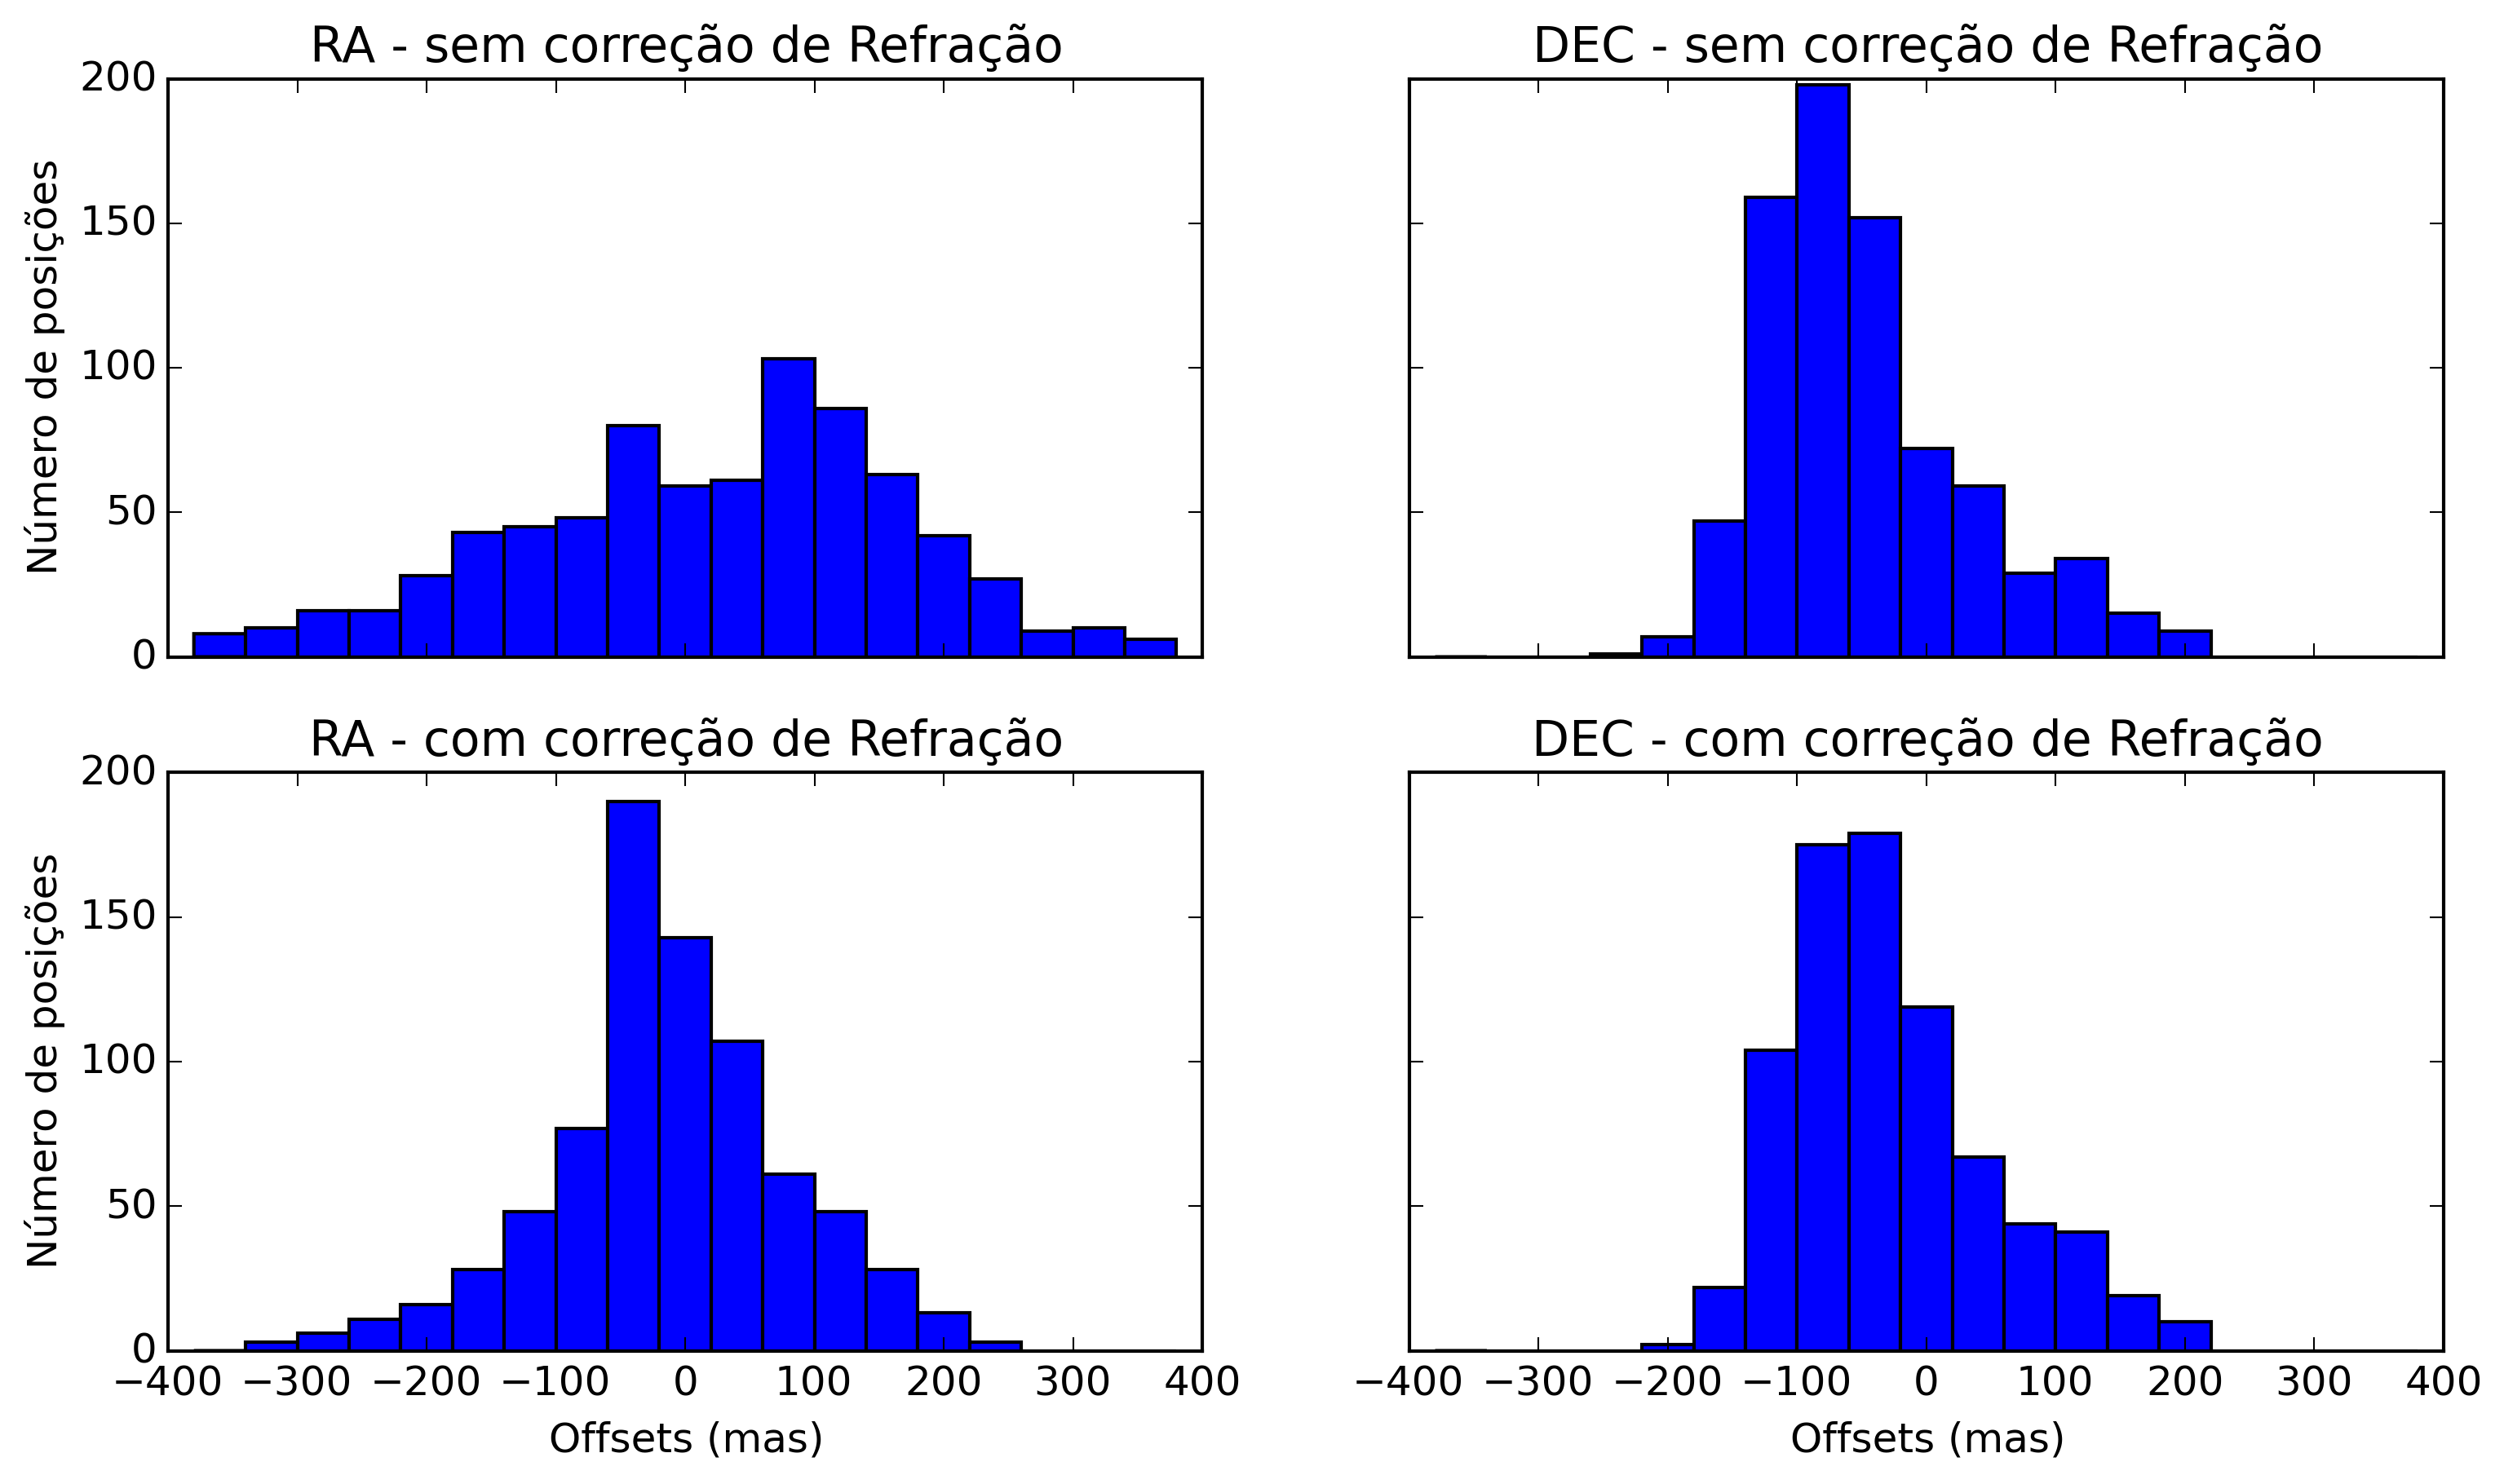
\includegraphics[width=16cm]{figuras/dist_Netuno_160.png} 
\caption{Distribuição dos offsets de Netuno observados no telescópio Perkin-Elmer no OPD antes e depois da correção de refração cromática. \label{Fig:refracao}}
\end{figure}

O segundo problema encontrado na posição de Netuno foi o fato dele ser aparentemente muito grande, maior que o seeing médio das estrelas. O ajuste com a gaussiana não se adequa muito bem ao topo da PSF de Netuno. Como Netuno está sempre bem amostrado, é possível que o ajuste da Gaussiana usando apenas as laterais da imagem de Netuno seja bom o suficiente. Porém para um ajuste completo, o Dr. Roberto Viera Martins desenvolveu uma PSF numérica para ajustar Netuno com melhor precisão.

A PSF numérica consiste em uma integral sobre um disco de raio R onde cada ponto no disco gera uma dispersão gaussiana de mesma largura à meia altura das estrelas da imagem. Outras características como escurecimento de bordo e ângulo de fase podem ser consideradas no cálculo.

Essa técnica está sendo testada em algumas posições de Netuno. O objetivo é verificar se o fotocentro calculado com a PSF numérica varia em relação à Gaussiana de forma significativa. Esse teste levará em conta o ângulo de fase da observação.

As posições finais a serem obtidas para o sistema Netuno-Tritão serão utilizadas em nova integração numérica que será realizada durante o meu doutorado sanduíche, o qual comecei em Setembro de 2016. Esse estágio tem duração de um ano e está sendo realizado no \textit{Institut de Méchanique Céleste et de Calcul des Éphémérides} (IMCCE) e é financiado pelo programa CAPES-COFECUB.

Essa nova integração numérica será usada para melhorar as efemérides de Tritão em relação a Netuno. Além disso, será possível analisar a efeméride de Netuno em relação ao Sol devido às diferenças das posições obtidas e das efemérides. Uma publicação é esperada desse trabalho.

Uma grande importância da melhoria na posição de Tritão é que está previsto para o dia 5 de Outubro de 2017 uma ocultação de uma estrela de magnitude R=12 por Tritão. A sombra prevista passará pela Europa e pela costa leste dos Estados Unidos e será uma grande oportunidade para estudar a atmosfera do satélite. Isso se torna mais significativo ao lembrar que Netuno está em uma região pouco densa de estrelas e ocultações são raras.


\chapter{Conclusão e Perspectivas}
\label{Cap: perspectivas}

\indent \indent Esse trabalho tem por meta estudar os objetos do Sistema Solar exterior, de forma a obter características físicas e dinâmicas relevantes para entender a formação e evolução do Sistema Solar. As técnicas utilizadas consistem em obter posições astrométricas precisas desses corpos para corrigir erros sistemáticos em suas efemérides, ou mesmo permitir a determinação de novas órbitas com novas integrações numéricas, a fim de melhorar a predição de futuras ocultações estelares.

Como participo ativamente em observações de TNOs e satélites com o objetivo de melhorar as efemérides e/ou predição de ocultações contribuí em mais 2 trabalhos. O primeiro sobra astrometria dos satélites internos de Urano publicado por \cite{Camargo2015}. O segundo sobre uma nova técnica de medidas relativas de grande precisão entre os satélites Galileanos \citep{Morgado2016}. Devido à grande quantidade de atividade desenvolvida em grupo, outras publicações em colaboração são esperadas. Também sou autor e co-autor de pôsteres e apresentações em congressos.

Além disso, no doutorado sanduíche, estou desenvolvendo, junto com o Dr. Valéry Lainey, pesquisador do IMCCE do Observatório de Paris, França, um código para integração numérica das órbitas de objetos do Sistema Solar. Esse trabalho é muito importante pois não existe no Brasil pessoas especializadas em integração numérica para geração de efemérides.

Um código próprio irá enriquecer o conteúdo de nossos trabalho dando um passo a mais além da publicação de posições astrométricas apenas. Isso também nos permitirá ter uma maior independência onde até agora precisávamos procurar uma colaboração.

Esse ano será suficiente para obter um código capaz de calcular órbitas de satélites irregulares, TNOs entre outros objetos, inclusive ajustando a órbita às observações. As observações de Tritão e Netuno serão utilizadas como teste.

Por fim, pretendemos observar ocultações estelares de satélites irregulares. Com o release do GAIA temos posições para as estrelas com precisão muito melhor às utilizadas até o momento. Além disso, trabalharemos na integração numérica das órbitas dos satélites, inclusive usando observações publicadas na literatura melhorando, portanto, suas predições.

\newpage
\bibliography{Referencias}
\bibliographystyle{apalike}


\end{document}
